%----------------------------------------------------------------------------------------
%       CHAPTER 18
%----------------------------------------------------------------------------------------

\cleardoublepage

\chapterimage{chx-cheerilee.png} % Chapter heading image

\chapter{FAQ}\label{ch:faq}

\hfill \break
\vspace{24mm}

\noindent \huge \textbf{\textit{aka}: 'Has this dumb question been asked before?'}\normalsize

%------------------------------------------------
\newpage
%------------------------------------------------

\section{Installation related questions}\label{faq:installation}

\vspace{2mm}

%------------------------------------------------
%

\subsubsection{Compiler errors}
\vspace{1mm}

Recent versions (ca. 10) of \texttt{gcc} (GNU C Compiler) may through up errors when compiling the \textbf{muffin} \textbf{netCDF} library routines -- '\texttt{Error: Rank mismatch ...}'.

\vspace{1mm}
This can be resolved by adding to \textsf{\footnotesize makefile.arc} (in \textsf{\footnotesize genie-main}):
\vspace{-1mm}\small\begin{verbatim}
FFLAGS += -fallow-argument-mismatch
\end{verbatim}\normalsize\vspace{-1mm}

%\vspace{1mm}
\noindent\rule{4cm}{0.5pt}
%------------------------------------------------
%

\subsubsection{Installation directory}
\vspace{1mm}

The default installation directory is:
\textsf{\footnotesize \(\sim\)/cgenie.muffin}
but it need not be. To run in \textsf{\footnotesize /NEW\_PATH}:
\vspace{1mm}

\begin{enumerate}[noitemsep]

\vspace{1mm}
\item Lines 26 and 27 of \textsf{\footnotesize user.mak}, change:
\vspace{1mm}
\vspace{-1mm}\footnotesize\begin{verbatim}
GENIE_ROOT        = $(HOME)/cgenie.muffin
OUT_DIR           = $(HOME)/cgenie_output
\end{verbatim}\normalsize\vspace{-1mm}
\vspace{1mm}
to:
\vspace{1mm}
\vspace{-1mm}\footnotesize\begin{verbatim}
GENIE_ROOT        = /NEW_PATH/cgenie.muffin
OUT_DIR           = /NEW_PATH/cgenie_output
\end{verbatim}\normalsize\vspace{-1mm}

\vspace{1mm}
\item Lines 31 and 34 of \textsf{\footnotesize user.sh}, change:
\vspace{1mm}
\vspace{-1mm}\footnotesize\begin{verbatim}
CODEDIR=~/cgenie.muffin
OUTROOT=~/cgenie_output
ARCHIVEDIR=~/cgenie_archive
LOGDIR=~/cgenie_log
\end{verbatim}\normalsize\vspace{-1mm}
\vspace{1mm}
to:
\vspace{1mm}
\vspace{-1mm}\footnotesize\begin{verbatim}
CODEDIR=/NEW_PATH/cgenie.muffin
OUTROOT=/NEW_PATH/cgenie_output
ARCHIVEDIR=/NEW_PATH/cgenie_archive
LOGDIR=/NEW_PATH/cgenie_log
\end{verbatim}\normalsize\vspace{-1mm}
\vspace{1mm}
... and, in \textsf{\footnotesize runmuffin.sh}, edit:
\vspace{1mm}
\vspace{-1mm}\footnotesize\begin{verbatim}
#####################################################################
# CHANGE THIS FOR INSTALLATIONS OTHER THAN IN $HOME
# SET THE SAME AS IN user.mak AND user.sh
# set home directory
HOMEDIR=$HOME
\end{verbatim}\normalsize\vspace{-1mm}

\end{enumerate}

%\vspace{1mm}
\noindent\rule{4cm}{0.5pt}
%------------------------------------------------
%
%
\subsubsection{Stack space}
\vspace{1mm}

You may encounter issues with regards to the \texttt{ifort} Intel FORTRAN compiler (an maybe others), particularly when using SEDGEM because of the size of the arrays holding sediment information:

\vspace{2mm}
\noindent ''\textit{The Intel® Fortran Compilers 8.0 or higher allocate more temporaries on the stack than previous Intel Fortran compilers.
Temporaries include automatic arrays and array sub-sections corresponding to actual arguments. If the program is not afforded adequate stack space at runtime relative to the total size of the temporaries,
the program will terminate with a segmentation fault.}''

\vspace{2mm}
\noindent The (a?) solution is to increase the CPU stack space, Try:
\vspace{-2pt}\small\begin{verbatim}$ ulimit -s unlimited\end{verbatim}\normalsize\vspace{-2pt}

%------------------------------------------------

\newpage

%------------------------------------------------

\section{Cluster/queue questions}

%------------------------------------------------
%
\subsubsection{Do I have to submit experiments to the queue rather than running interactively?}

\textbf{Yes!} Except for developing the model and debugging, testing new experimental designs, and forcing a re-compile. The number of instances of the model that can be run simultaneously interactively is limited by the number of processing cores on the head node. The more experiments that are run interactively, the slower everything will go. Additionally, if you even temporarily lose your Internet connection, an interactively-run experiment will die. The queue is there for your convenience, believe it or not ...

%------------------------------------------------
\subsubsection{Can I leave all my experiment results on the cluster for ever?}

\textbf{No!} \uline{Nothing} is backed up on the cluster, and space is not infinite. So, periodically, transfer archived (\texttt{.tar.gz}) results off of the cluster and delete both the archive file and the results directory.

%------------------------------------------------

\newpage

%------------------------------------------------

\section{Help! My experiment has died ... why?}

%------------------------------------------------
%

%------------------------------------------------

\subsection{Sources of initialization error}

If, when using the \textsf{\footnotesize runmuffin.sh} shell script to run a \textbf{cgenie.muffin} experiment, it all goes horribly pear-shaped ...
\vspace{1mm}
\begin{enumerate}

\vspace{1mm}
\item The experiment dies absolutely immediately.
\\Check that the \textsf{\footnotesize runmuffin.sh} shell script has executable permissions. Also check that the directory you are trying to run the model from is the \textsf{\footnotesize genie-main} directory.

\item The experiment does not quite die immediately, but does not manage to stagger even as far as the line:
\vspace{-4pt}\begin{verbatim}
>> Here we go ...
\end{verbatim}\vspace{-4pt}
before dropping dead. If so, there should be an error message telling you that a particular file or directory cannot be found. Check:

\begin{itemize}
\item All the files and directories you have specified exist.
\item You have not omitted spaces where you should not have, nor added spaces where a '\texttt{\_}' separator was required.
\item You have not misspelt anything -- a common cause of problems is in reading the number one ('\texttt{1}') for the letter el ('\texttt{l}'), or \textit{vice versa} in the computer font (\texttt{Courier}).
\end{itemize}

\end{enumerate}
\vspace{2mm}

\noindent These first two sorts of pain and suffering are due to mis-configuration of the \textsf{\footnotesize runmuffin.sh} shell script. Also refer back to the overall sequence of configuring and running the \textbf{cGENIE.muffin} model shown in Figure \ref{fig:chx-jobcreation}.

\noindent Other sources of error are due to the configuration of \textbf{cGENIE.muffin} (or more rarely, due to the model itself):

\vspace{1mm}
\begin{enumerate}

\vspace{1mm}
\item As \textbf{cGENIEmuffin} initializes, files may be reported as not being found. One possible cause of this is that '\texttt{\~{}}' may not necessarily get expanded into the path of your home directory (e.g., '\texttt{/home/mushroom}'. In this situation, '\texttt{\~{}}' can simply be replaced with '\texttt{\$HOME}'. Note that as well as making this substitution at the command line, the \textit{user-config} file may also contain instances of '\texttt{\~{}}' (such as in specifying particular \textit{forcings}).

\vspace{1mm}
\item A missing/not found error can also arise with some compilers if one of the various ASCII input files to \textbf{BIOGEM} (or \textbf{SEDGEM}) does not have a blank line at the bottom (some vague quirk of the unformatted read used in the \textbf{FORTRAN} code). Check: the \textit{user-config} file, and also any boundary condition files being requested.

\vspace{1mm}
\item Further trouble can occasionally arise when using \textbf{Windoz} and editing files (e.g., the \textit{user-config} file) and it is possible to corrupt the format of the file. For what file(s) you have edited, use the command \texttt{dos2unix} to strip off \textbf{Windoz} formatting characters (which are invariably invisible in most editors). The syntax for this (or see the \textbf{linux} 'man' pages, or even Google it) is \texttt{\$ dos2unix FILENAME}.

\end{enumerate}
\vspace{2mm}

%------------------------------------------------
%
\newpage
\subsection{Carbonate chemistry errors}

The most common error as \textbf{muffin} starts to run, or during the course of a run relates to the solution of the aqueous carbonate chemistry  system and specifically, for \(pH\). There are 2 different errors that can be reported in this respect:

\begin{enumerate}[noitemsep]

\vspace{2mm}
\item 
\small\begin{verbatim}
Numerical instability at step; ...
Data; dum_DIC,dum_ALK,dum_Ca,dum_SO4tot,dum_H2Stot,dum_NH4tot
pH(SWS), pH (OLD), pH (guess #1), pH (guess #2)
CARBONATE CHEMISTRY COULD NOT BE UPDATED :(
\end{verbatim}\normalsize
followed by a series of values (corresponding to the listed tracers), and then a block of text summarizing possible meanings of the error (and tracer values).

\vspace{2mm}
\item 
\small\begin{verbatim}
Number of steps taken without successfully solving for pH = ...
Data; dum_DIC,dum_ALK,dum_Ca,dum_SO4tot,dum_H2Stot,dum_NH4tot
pH(SWS), pH (OLD), pH (guess #1), pH (guess #2)
CARBONATE CHEMISTRY COULD NOT BE UPDATED :(
\end{verbatim}\normalsize
also followed by tracer values and possible explanations.
\end{enumerate}

\vspace{1mm}
\noindent Both errors relate to the implicit solution for the \(pH\) (technically: \([H^{+}]\)) value at the current time-step. The scheme takes an assumed value at model initialization or from a re-start, or during an experiment -- the last calculated value at that location in the ocean, and uses this to make an updated estimate of \(pH\). The calculation is carried out iteratively, with the new assumed value of \(pH\) being taken from the previous iteration, until the solution converges, or not.

The first error -- instability -- is triggered by a negative value of \(pH\) being calculated. The second  (much more common) error occurs if the maximum number of iterations has been reached -- i.e. if the carbonate chemistry system is not converging within a reasonable number of iterations. \footnote{The default number of iterations is set as \(100\) and is specified by the parameter: \texttt{gm\_par\_carbchem\_pH\_iterationmax=100}}

The default behavior in response to either situations occurring is for muffin to forego updating \(pH\) in the troublesome ocean grid call and continue to the end of the current time-step, save data snapshot, and then exit the run.

\vspace{1mm}
Why does the error arise, and what can be done about it?

\begin{enumerate}[noitemsep]

\vspace{2mm}
\item 
Running \textbf{muffin} with array dimensions which do not match the number of tracers selected is a common cause of failures to solve the aqueous carbonate system, as often calcium ion or other tracer concentrations become corrupted and get assigned nutty values.  
\\As per the error message text:
\small\begin{verbatim}
(1) Check the FIRST TWO lines of the ERROR DATA (ocean DIC and ALK):
    -> These should be ... reasonable ... of order a few thousand umol kg-1
       (units reported are mol kg-1)'
    -> NaNs, negative values, obsenely low (<< a few hundred umol kg-1) or,
       high (>> tens of thousands) are indicative of array bounds problems.
       Array bounds problems are mostly commonly due to:
       (A) incorrect ocean dimension compared to the compiled executable,
       (B) incorrect number of biogeochem tracers in the ocean compared to
           the compiled executable.
    => Carry out a *** make cleanall *** (from ~/genie/genie-main). 
(2) ...
(3) Extreme values of Ca and SO4 (#3, #4) are only vanishingly possible except
    due to incorrect compiled array dimension or extreme salinity.
\end{verbatim}\normalsize
Try forcing a re-compile (\texttt{\$ make cleanall}) to make this go away.
\vspace{1mm}
\\Also, if a \textit{re-start} is used which was generated with a different land-sea mask (and \textit{base-config}) to the current experiment and associated \textit{base-config}, spurious tracer values can occur and crash the carbonate chemistry scheme. Try running without the \textit{re-start} and see if that solves it (identifies the source of the problem).

\vspace{1mm}
\noindent The appearance of all (or almost all) \texttt{NaNs} also hints at a ocean circulation/climate model component problem and only causes an immediate crash in the ocean carbonate chemistry. One not infrequent cause is due to the sea-ice model that is not unconditionally stable and when it fails, can lead to \texttt{NaN} tracer concentrations. In particular, the sea-ice model can fail when there is very little sea-ice cover -- either retreating or increasing -- and in topographically restricted regions (e.g. small embayments or semi-enclosed seas at high latitudes). If the sea-ice model fails, this should be recorded in a series of error messages notifying a failure to solve. Check the experiment log file if running submitted jobs.\footnote{Interactive jobs should echo the error messages to the screen as the failure occurs.}

\vspace{1mm}
If the root of the issues is indeed the sea-ice model, one or more of the following can be tried:

\begin{itemize}[noitemsep]

\vspace{1mm}
\item Simply run the model 'warmer' (higher \(pCO_{2}\) or radiative forcing) so that there is no sea-ice cover anywhere, or 'colder' so that there is plenty. (It seems to be the appearance or disappearance of an ephemeral sea-ice cover that is the main issues.)
\noindent If not running from a \textit{restart}, you can also try specifying a 'warmer' or 'colder' ocean start than the default. The initial ocean temperature of a spin-up is determined by the parameters (set in the \textit{base-config} although you can add new values in the \textit{user-config}):
\vspace{-1mm}
\vspace{-0pt}\small\begin{verbatim}
# temp0 -- ocean temperature start
go_10=5.0
# temp1 -- start temperature start
go_11=5.0
\end{verbatim}\normalsize\vspace{-0pt}
\vspace{-1mm}
(Aim to set both parameters to the same value because I have forgotten what the difference between them is ... (vertical zones of temperature perhaps).)
\vspace{1mm}
\item Check that you have the revised sea-ice diffusivity value and limits imposed on sea-ice advection, set by (this also appears in the \textit{base-config} but you can adjust the values in the \textit{user-config}):
\vspace{-1mm}
\vspace{-0pt}\small\begin{verbatim}
# reduced sea-ice eddy diffusivity
gs_11=1000.000
# set a fractional sea-ce coverage threshold for preventing advection
gs_par_sica_thresh=0.99
\end{verbatim}\normalsize\vspace{-0pt}
\vspace{1mm}
\item The nuclear option(!) is to disable the formation of sea-ice entirely, which can be done via:
\vspace{-1mm}
\vspace{-0pt}\small\begin{verbatim}
eb_opt_freeze=.false.
\end{verbatim}\normalsize\vspace{-0pt}
\vspace{-1mm}
(This simply sets the freezing point of seawater to -999C and hence preserves the water and energy balance of the system.)

\end{itemize}

\vspace{2mm}
\item Failure to converge (the second error) is unlikely to be due to mis-compiled tracer selections or incomparable restart ocean grids, but rather as a consequence of extreme geochemical conditions occurring somewhere in the ocean. This can be due to excessively intense export production and remineralization, as well as at excessively high dissolved silica concentrations -- all may be plausible early Earth states, but ones that require an adjustment of how aqueous carbonate chemistry is solved:

\begin{itemize}[noitemsep]
\vspace{1mm}
\item At very high nutrient (\(PO_{4}\)) concentrations, and/or at high ocean temperatures with a temperature-dependent remineralization scheme, and/or with a slow prescribed sinking speed\footnote{i.e. much slower than the default of \(125 md^{-1}\)}, oxygen consumption can be complete and subsequently, sulphate reduction intense. Sulphate reduction results in the release of two mol alkalinities per mol \(SO^{2-}_{4}\) consumed, impacting carbonate chemistry in that ocean cell (in addition to the release of \(DIC\) from the remineralized organic matter). Where the resulting \(H_{2}S\) is re-oxidized, alkalinity is removed and local carbonate chemistry impacted in the opposite sense.
\\The problems are likely to occur in the ocean sub-surface, although difficulties at the surface and associated with air-sea gas exchange are also possible. Plotting out surface or sub-surface (and ideally; 2D surfaces of the distribution of minimum and maximum values using \textbf{muffinplot}) can help in the identification of the nature of the underlying problem(s).
\\There are a couple of possible courses of action to take (as an alternative to modifying the experimental design and reducing the intensity of biological export and sub-surface recycling):
\begin{enumerate}[noitemsep]

\vspace{1mm}
\item Increase the number of iterations allowed in solving for seawater \(pH\).
\footnote{Conversely, one could decrease the \(pH\) tolerance criteria for convergence: \texttt{gm\_par\_carbchem\_pH\_tolerance}, which by default has a value of \(0.001\) -- increasing will result in a faster solution and a greater change of passing the convergence criteria, but at the expense of accuracy.}
The parameter controlling this is:
\vspace{-0pt}\small\begin{verbatim}
# number of pH solution iterations
gm_par_carbchem_pH_iterationmax=100
\end{verbatim}\normalsize\vspace{-0pt}
and could, for instance, be increased to a value of \(1000\) (iterations).

\vspace{1mm}
\item In addition to the \(100\)\footnote{The default value unless it has been changed.} iterations that \textbf{muffin} is allowed in trying to converge on a solution for \(pH\), \textbf{muffin} can also try a different initial (seed) \(pH\) value if it encounters one of the error conditions. The iteration counter is re-set and the iterative convergence calculation is carried out once again. 
\\The controlling parameter is:
\vspace{-0pt}\small\begin{verbatim}
# re-seed pH?
gm_ctrl_carbchem_pHseed_retry=.false.
\end{verbatim}\normalsize\vspace{-0pt}
and is \texttt{false} by default.
\\In a situation by which \(pH\) never ever converges, it may be that the initial value is too far from the (true) solution value. Setting the parameter \texttt{true} and re-seeding with randomly varying values then help find a sufficiently close initial guess that convergence occurs.

\vspace{1mm}
\item Whilst the carbonate chemistry and \(pH\) at the ocean surface is solved at every time-step (in order to calculate air-sea gas exchange of \(CO_{2}\), carbonate chemistry is not needed for any reaction, with the exception of when one or more of the following \textit{tracers} are selected:
\vspace{1mm}
\begin{itemize}[noitemsep]
\item \texttt{is\_FeCO3}
\item \texttt{is\_Fe3Si2O4}
\item \texttt{io\_CH4}
\end{itemize}
\vspace{1mm}
(Carbonate chemistry is also needed for calculating the preservation of \(CaCO_{3}\), but this is calculated separately in \textbf{SEDGEM}.)
\\The error then arises most likely when an attempt to solve for \(pH\) is made when preparing 3D fields for \textit{time-slice} saving. This calculation is made regardless of whether or not you want carbonate chemistry \textit{time-slice} data saved. An option is available that disables the updating of \(pH\) associated with \textit{time-slice} saving:
\vspace{1pt}\small\begin{verbatim}
# disable carbonate chemistry updating for time-slices
bg_ctrl_data_save_slice_carb_update=.false.
\end{verbatim}\normalsize\vspace{1pt}
(by default, this parameter is \texttt{.true.}).
Aside from at the surface every time-step, employing this parameter change results in the ocean interior \(pH\) only being solved for at the very start of the experiment. Carbonate chemistry \textit{time-slice} data is still saved ... but will not change from the initialised values (except at the surface).
\\This *should* avoid most/all carbonate chemistry crash issues(?)

\vspace{1mm}
\item You could also try forcing \(pH\) to be solved for, throughout the ocean interior, and at every single time-step. This might 'work', because the \(pH\) solution is seeded with the previous \(pH\) value, meaning that very frequently updating the value of \(pH\) might allow you to track the transition into extreme redox states with no issues. The parameter setting to make this happen is:
\vspace{-0pt}\small\begin{verbatim}
# force full carbonate chemistry updating
bg_ctrl_carbchemupdate_full = .true.
\end{verbatim}\normalsize\vspace{-0pt}
Note that if you have a methane cycle, ocean interior \(pH\) is frequently solved for anyway.

\end{enumerate}
\vspace{1mm}

Option (c) is arguably the better one to test first, unless you have a methane cycle. Then (d) is worth trying (but even if it works, may slow things down). Otherwise, (a) and (b) may help but will probably only offer limited improvement in stability.

\vspace{1mm}

There is a fifth and slightly different, possibility, requiring the marine carbon cycle itself is altered:

\begin{enumerate}[noitemsep]
\vspace{1mm}
\item[(e)] Assuming that the underlying issue is 'nutrient trapping' -- the rapid biological removal of (\(PO_{4}\)) from the surface, following by shallow remineralization of the organic matter, re-release of the (\(PO_{4}\)) and then efficient return back to the surface to fuel further biological productivity -- adding \(Fe\) co-limitation of biological productivity may help, because loss of dissolved \(Fe\) from the water column will tend to scale with the flux of organic matter, hence acting as a negative feedback on the nutrient trapping. 
\end{enumerate}

\vspace{2mm}
\item Very high\footnote{Orders of magnitude higher than modern} high dissolved silica (\(H_{4}SiO_{4}\)) concentrations in the ocean can cause issues. This is because \(H_{3}SiO^{-}_{4}\) appears in the calculation of carbonate alkalinity from total alkalinity.
\\A parameter is provided to remove \(H_{3}SiO^{-}_{4}\) from the alkalinity carbonate calculation -- by setting:
\vspace{-1pt}\small\begin{verbatim}
gm_ctrl_carbchem_noH3SiO4=.true.
\end{verbatim}\normalsize\vspace{-1pt}

\end{itemize}

\end{enumerate}

\vspace{1mm}
\noindent\rule{4cm}{0.5pt}
\vspace{2mm}

\noindent You may also be trying to spin up the model with fabulously high \(pCO_{2}\) (i.e. many \(10s\) or even \(100s\) of thousands of \(ppm\)). What typically happens here, is that mean ocean \(DIC\) and \(ALK\) are invariably initialized to modern (or shallow time) values, in equilibrium with modern (or up to \(1000 ppm\)) \(pCO_{2}\). Restoring the atmosphere to an excessively high \(pCO_{2}\) will lead to extreme imbalances between \(DIC\) and \(ALK\) at the ocean surface as \(CO_{2}\) invades the ocean from the atmosphere.

If you do not need to simulate \(pH\) or carbonate saturation state, or are not using processes that depend on these (e.g. variable saturation-dependent \(CaCO_{3}:POC\) rain ratios, or the preservation of \(CaCO_{3}\) in deep-sea sediments, then you might consider setting a radiative forcing in the atmosphere equivalent to the required \(pCO_{2}\) value, and just let \(pCO_{2}\) naturally equilibrate with ocean \(DIC\) and \(ALK\) (and the climate and biological pump state).  

\vspace{1mm}
If you really *must* have an explicitly high value of \(pCO_{2}\), then you can try one of the following, with the aim to set ocean \(ALK\) to a more appropriate value:

\begin{enumerate}[noitemsep]

\vspace{1mm}
\item Firstly you can estimate the initial mean ocean \(ALK\) value you need from an off-line carbonate chemistry code. 
\\Typical would be to assume a modern ocean surface saturation state with an \(\Omega\) of calcite of around \(5.0\) (mean ocean saturation is \(5.06\) in the modern configuration of \textbf{muffin}). Take a reasonable mean ocean surface temperature and salinity ... and an atmospheric partial pressure equal to the value you want to restore to, and then solve for the complete (mean surface) system. Initialize your experiment with the resulting \(DIC\) and \(ALK\) values.

\vspace{1mm}
\item Read suitable \(DIC\) and \(ALK\) values off of Figure \ref{fig:fan1}.
\\This is far from a particularly great figure and is poorly resolved in terms of \(pCO_{2}\) (black) and saturation (\(\Omega\)) (yellow) contours. You are looking to follow the \(pCO_{2}\) contour you want (or close to), to higher ocean \(ALK\), until the ocean surface is reasonably over-saturated (i.e. \(1.0<\Omega<10.0\)). e.g. for \(\times10\:pCO_{2}\), this would occur for an \(ALK\) value of ca. \(5\:mmolkg^{-1}\). You also want to read off a corresponding \(DIC\) value, which you could simply take to be the x-axis value (but noting that this is really \(DIC\) \uline{plus} \(pCO_{2}\)).

\vspace{1mm}
\item Restore ocean carbonate chemistry (e.g. surface ocean saturation) at the same time as you restore atmospheric \(pCO_{2}\).
\\Refer to the \textbf{Forcing HOW-TO}, and specifically: '\textit{Set a specific ocean chemistry or saturation state}'. The 3rd listed method is the one you want.
\\In this method, you might have to ramp up \(pCO_{2}\) to its eventual, required value, rather than implementing an instantaneously high \(pCO_{2}\) value.

\end{enumerate}


\begin{figure}
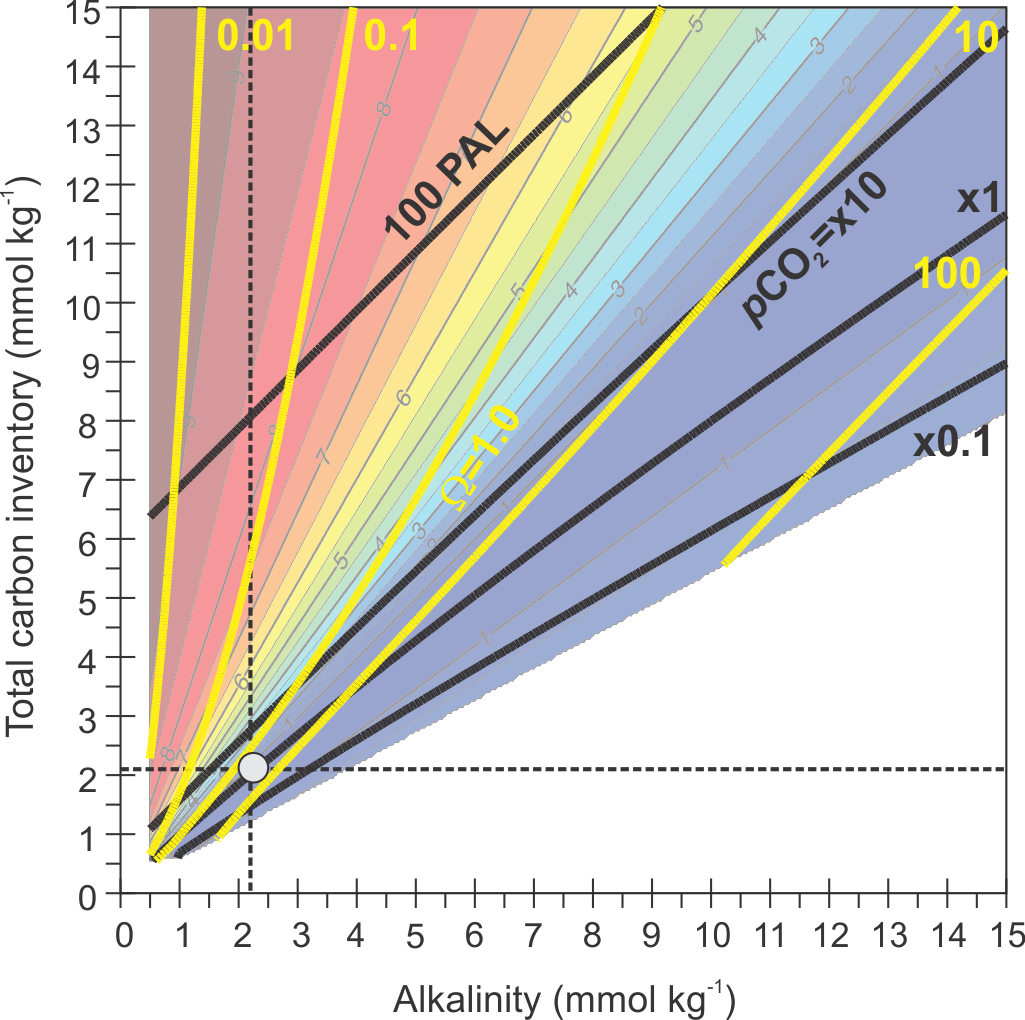
\includegraphics[width=0.7\textwidth]{fan1.png}\centering
\vspace{-0mm}
\caption{Carbonate chemistry fan diagram (at \(15^{\circ}C\)).\\Note that the total carbon inventory is the sum of both \(DIC\) and \(pCO_{2}\). The circle represents mean modern ocean chemistry.}
\label{fig:fan1}
\end{figure}


%------------------------------------------------
%
\newpage

\subsection{Other possible geochemical errors}

It is good practice not to allow complete consumption of any particular reactant by a single reaction. This is because multiple processes may be competing for the same reactant, whilst at the same time, ocean circulation is transporting the reactant away. The result can be (small) negative tracer values (and if you are unlucky, large negative errors). Negative tracer value, in turn, have the potential to cause crashes.

A parameter is hence provided to limit the maximum consumption of any particular reactant by a single reaction via an imposed lifetime (days): 
\small\vspace{-1mm}\begin{verbatim}
# maximum time-scale to geochemical reaction completion (days)
bg_par_bio_geochem_tau=90.0
\end{verbatim}\vspace{-1mm}\normalsize

\noindent In this example, the value is set to \(90\:d\).\footnote{By default it is set to zero which is interpreted as allowing complete reactant consumption as per previously.}

\vspace{1mm}
\noindent\rule{4cm}{0.5pt}
\vspace{2mm}

\noindent Negative tracer values can also arrise as a result of the default ocean mixing scheme. In all modern and 'realistic' paleo configurations, isopycnal/diapycnal mixing is used. However, this scheme can lead to unwanted negative tracer values. In extreme biogeochemical configurations, particularly at low atmospheric \(pO_{2}\) and when sharp horizontal transitions in redox state in the ocean occur, the magnitude of negative values can become unacceptable.

An option is provided for toggling between isopycnal/diapycnal (\texttt{.true.}) and horizontal/vertical (\texttt{.false.}) mixing schemes. For instance, adding:
\small\vspace{-2pt}\begin{verbatim}
# it is recommended that it is turned OFF (=.false.) for 'fake' worlds
go_diso=.false.
\end{verbatim}\vspace{-2pt}\normalsize
would request the horizontal/vertical mixing scheme and substantially reduce the possibility of negative tracer values arising.

%------------------------------------------------
%
\newpage

\subsection{Meaning of specific error and warning messages}

\vspace{2mm}
\subsubsection{'ERROR: path integral around island too long'}

Such an error is possible when developing new or modifying existing continental configurations (and associated 'island' and 'path' definition files), but not in normal running of the model.
First try a \texttt{make cleanall} and then try re-running.
If the problem persists, it is possible that a key configuration file has accidently/somehow been changed.

\vspace{2mm}
\subsubsection{'ERROR MESSAGE: Particulate tracer CaCO3 ...'}

I have been told '\texttt{ERROR MESSAGE: Particulate tracer CaCO3 does does not have the corresponding ocean tracer Ca selected}' -- is this a problem ... ?

\textbf{No!} You are simply being reminded that you have calcium carbon (CaCO$_{3}$) selected as a particulate tracer in the model, but although when it dissolves it releases Ca$^{2+}$ (and removes Ca$^{2+}$ when CaCO$_{3}$ is precipitated), you do not have Ca$^{2+}$ selected as an explicit dissolved tracer in the ocean. This is not a problem as by far the most important effect on the carbon cycle of adding/subtracting Ca2+ is a change in alkalinity, which is implicitly account for. Only on \textbf{very} long time-scales, or in deep-time situations when the Ca$^{2+}$/Mg$^{2+}$ ratio was very different form today, might you need to select Ca$^{2+}$ (and Mg$^{2+}$) as an ocean tracer.

%------------------------------------------------

\newpage

%------------------------------------------------

\section{General model experiment questions}

%------------------------------------------------
%
\subsubsection{When does the model need to be recompiled?}

\textbf{cGENIE.muffin} will need to recompile in the following situations:

\begin{itemize}

\vspace{1mm}
\item You have just carried out one of the \textbf{cGENIE.muffin} tests, e.g., \texttt{make test} or \texttt{make testbiogem}.
\item You have changed the dimension of the climate model grid (which also means an automatic change in the biogeochemistry modules), either horizontally (e.g., going from \(36\times 36\) to \(18\times 18\)) or vertically (e.g., going from \(8\) levels in the ocean to \(16\)).
\item You have changed the number of selected ocean biogeochemical tracers in the \textit{base-config} and hence changed the value of:
\small\begin{verbatim}
GOLDSTEINNTRACSOPTS='$(DEFINE)GOLDSTEINNTRACS=2'
\end{verbatim}\normalsize

\end{itemize}
(The latter two involve a change in compiled array dimension.)

In all three situations, the \textit{base-config }is being changed (or should be\footnote{One could edit a \textit{base-config} and re-ruin, but it is better to create a new \textit{base-config }file if editing any of the settings, particularly those affecting array dimensions}). In running at the command line (i.e. interactively), the \texttt{\footnotesize runmuffin.sh} script detects the change in base-config, and automatically forces a re-compile for you. However, the compute nodes of the cluster do not have access to the \textbf{FORTRAN} compiler. As a sad and unfortunate consequence, submitted jobs cannot recompile modules and all science modules must be already compiled when a job is submitted.\footnote{It is OK to change the flavor of GENIE as linking is done by the C compiler.}

To  recompile (and re link) the science modules -- first, start an interactive run of the experiment you want to conduct. This will ensure that it is correctly compiled. This also serves as a visual check that you have requested a \textit{user-config}, restart, etc that actually exists. Start the run for the length of time you intend to use when submitting the experiment as a job to the queue, but kill it (keyboard command: \textsf{\footnotesize Ctrl-C}) once it is compiled and you are happy that it is running OK (say, after 10 years).
\noindent You can now be reasonably confident that the experiment is safe to submit the job to the cluster (and all files and inputs are as they should be).

If you have multiple experiments, all with the same resolution and number of tracers, you DO NOT need to re-run interactively or attempt to recompile. Also, you can add 'modules' and not recompile. i.e., you can interactively run an ocean -only carbon cycle. And then submit it. And then submit an experiment using \textbf{SEDGEM} as well. (Because when the model is compiled, ALL sciences modules are compiled, meaning that all there is to do is just link them, which does not require the (\texttt{ifort}) \textbf{FORTRAN} compiler.)

Refer to Figure \ref{fig:chx-jobcreation} for the sequence of steps associated with configuring and running model experiments.

%------------------------------------------------
%
\subsubsection{In the naming of different \textit{forcing} specifications: what does '\texttt{yyyyz}' mean?}

\textbf{A.} The naming convention for \textit{forcings} is that the (sub)directory name starts with the code for the continental configuration, if the \textit{forcing} is tied to a specific continental configuration. For example: \textit{forcings} with the string '\textsf{\footnotesize FeMahowald2006}' relate to the prescription of a dust (Fe flux) field re-gridded from \textit{Mahowald et al.} [2006]. When this has been re-gridded to the \textsf{\footnotesize worjh2} continental configuration, \textsf{\footnotesize worjh2} appears at the start of the name. If the \textit{forcing} is independent of a specific continental configuration, such as restoring atmospheric \(CO_{2}\) to a prescribed value (uniformly throughout the atmosphere), the string is '\textsf{\footnotesize yyyyz}', as in e.g.: \textsf{\footnotesize pyyyyz\_Rp\(CO_{2}\)\_Rp13\(CO_{2}\)}.

%------------------------------------------------
%
\subsubsection{Can I make the model run faster?}

*sign* You speed freak. Is this all you care about? What about the quality of the simulation - does that mean absolutely nothing to you? Oh well ...
There is a bunch of stuff that slows \textbf{cGENIE.muffin} down that may not be absolutely essential to a particular model experiment. These include:

\begin{itemize}[noitemsep]
\setlength{\itemindent}{.2in}

\item   The number of tracers - if you don't need 'em, then don't select 'em! Selected tracers are automatically passed to \textbf{GOLDSTEIN} and advected/convected/diffused with ocean circulation. Similarly, \textbf{BIOGEM} does a whole bunch of stuff with tracers, particularly those which can be biologically transformed. All this is numerically wasteful if you aren't interested in them. Equally importantly, the more tracers you have selected the more careful you have to be in configuring the model. Superfluous tracers therefore cost more configuration time and/or increase the change of a model crash.

\item \textit{Tracer auditing} - the  continuous updating and checking global tracer inventories to ensure that there is no spurious loss or gain of any tracer (i.e., a bug) has computational overheads associated with it. Whether this checking is carried out or not is set by the value of the flag \texttt{bg\_ctrl\_audit}\footnote{It is \texttt{.false.} by default.}.

\item \textit{Time-series} results saving. Model tracer (plus some physical) properties are bring continuously averaged in constructing \textit{time-series} results files. Cutting down on \textit{time-series} that you don't need will help minimize model run-time. The various categories of time-series that will be saved are specified by a series of namelist parameter flags. However, within each category (such as \texttt{ocn} tracers - \texttt{bg\_ctrl\_data\_save\_sig\_ocn}) all properties will be saved - you are not given to option to save a defined sub-set (for example, \(DIC\) and \(PO_{4}\) in the ocean but not \(ALK\)).

\item Time-slice results saving. If you have relatively few requested time-slices over the course of the model integration then this is unlikely to significantly impact the overall run-time (even will all possible data category save namelist flags set to \texttt{.true.}). However, note that if you have accidently triggered the default time-slice saving interval (by having no data items in the time-slice specification file (\texttt{bg\_par\_infile\_slice\_name}) you may end up with the model running about as fast as a 2-legged dog super-glued to a 10-tonne biscuit.

 Note that time-series saving of data that is a 2-D average, such as atmospheric composition at the ocean-atmosphere interface, sediment composition at the ocean-sediment interface, or just ocean surface conditions, is less numerically demanding than mean values that have to be derived from a 3-D data field.

\item Alter the degree of synchronicity between climate and biogeochemistry (see  HOW-TO guide).

\end{itemize}

\vspace{2mm}
As a very rough guide, the impact on total run-time of making various changes to the model configuration are listed as follows. Numbers are given as a percentage increase in total model run-time (using the /usr/bin/time linux command). Tracers selected in the ocean are DIC, ALK, PO4, O2, DOM\_C, DOM\_P, DOM\_O2, as well as 13C isotopic components (DIC\_13C and DOM\_C\_13C) (+ T and S). The corresponding tracers are present in the atmosphere and as particulates. The model is run for 10 years as a new run (i.e., not loading in a restart file):

\begin{itemize}[noitemsep]
\setlength{\itemindent}{.2in}

\item   ADD auditing \begin{math}\Rightarrow\end{math} +15\%
\item   ADD time-slice saving   \begin{math}\Rightarrow\end{math} +20\%\footnote{Because only a 10 year integration has been carried out with a time-slice saved at 10 years, the computational cost of time-slice saving is disproportionately high as displayed. With a longer integration, the relative cost of saving a time-slice will fall. In contrast, the computational cost as a fraction of total run-time of time-series saving and auditing is likely to remain the same.}
\item   ADD time-series saving  \begin{math}\Rightarrow\end{math} +15\%
\item   REMOVE \begin{math}^{13}\end{math}C isotopic species (= DIC and DOC ocean tracers) \begin{math}\Rightarrow\end{math} -10\%\footnote{The speed gained by removing two tracers is not proportional to the fractional decrease in number of tracers (in this example reducing from 11 to 9 the number of tracers in the ocean gives only a ca. 10\% improvement in overall speed).}

\end{itemize}

\vspace{2mm}
You can also run at lower resolution. The basic configuration for a faster 'lego box' \textbf{cGENIE.muffin} configuration consists of a \(18\times 18\) model grid and an \(8\) level ocean. The continents are in a zonally-averaged configuration and there is no topography in the oceans.

The model is accelerated by:

\begin{enumerate}[noitemsep]
\setlength{\itemindent}{.2in}
\item it's low resolution
\item taking \(48\) instead of \(96\) ocean time-steps per year in the ocean
\item \textbf{BIOGEM} being only being updated every \(4\) rather than every \(2\) ocean time-steps.
\end{enumerate}

In this configuration 100 years take about 40 seconds, 10 kyr would just take over and hour, and 100 kyr could be run overnight!

%------------------------------------------------

\newpage

%------------------------------------------------

\section{Climate-y questions}

%------------------------------------------------
%
\subsubsection{Can I disable climate feedback with \(CO_{2}\)?}

Yes, for instance when you might want to compare the fate of \(CO_{2}\) released to the atmosphere with climate (and ocean circulation and temperatures) not responding, vs. \(CO_{2}\) in the atmosphere also driving changes in climate (and hence affecting the pathways and transformations of \(CO_{2}\), particularly in the ocean).

\vspace{2mm}
To specify no climate feedback, add to the \textit{user-config} file:
\vspace{-2mm}\small\begin{verbatim}
# set no CO2 climate feedback
ea_36=n
\end{verbatim}\normalsize\vspace{-2mm}
as well as a radiative forcing scaling:
\vspace{-2mm}\small\begin{verbatim}
# scaling for atmospheric CO2 radiative forcing, relative to 278 ppm
ea_radfor_scl_co2=1.0
\end{verbatim}\normalsize\vspace{-2mm}
(a value of \texttt{1.0} giving no change in climate relative to the default).

%------------------------------------------------
%
\subsubsection{How does the fresh water flux adjustment work?}

Without a dynamical atmosphere and sufficient resolution e.g. North American topography, the EMBM atmospheric component component produces an overly weak net transport of fresh water from the North Atlantic into the North Pacific -- too weak to maintain an AMOC (how sad).

A fix is provided in the form of a prescribed transport of fresh water from the Atlantic to Pacific (or salt from the Pacific to Atlantic). The transport is split up into 3 zones\footnote{Also see notes in the xml parameter definition in addition to description below and references.} -- approximately:

\vspace{1mm}
\begin{enumerate}[noitemsep]
\item South Atlantic into the (South) Pacific
\\\noindent [latitude band \texttt{j=9,12} (\texttt{36x36} grid)]
\item Equatorial and southern subtropical Atlantic into the Pacific
\\\noindent [latitude band \texttt{j=13,25} (\texttt{36x36} grid)]
\item North Atlantic (and Arctic) into the North Pacific
\\\noindent [latitude band \texttt{j=26,36} (\texttt{36x36} grid)]
\end{enumerate}
\vspace{1mm}
See Figure 1 in \textit{Marsh et al.} [2004] (\textit{Climate Dynamics}) for an illustration. By default [\textit{Edwards and Marsh}, 2004], the fluxes combine for a total net transfer of 0.32 Sv following Oort [1983] and individually are (with parameter name):
\vspace{1mm}
\begin{enumerate}[noitemsep]
\item (xml name: \texttt{extra1a}) \texttt{ea\_25=-0.03}
\item (xml name: \texttt{extra1b}) \texttt{ea\_26=0.17}
\item (xml name: \texttt{extra1c}) \texttt{ea\_27=0.18}
\end{enumerate}
\vspace{1mm}
and giving a total net flux adjustment (\texttt{extra1a+extra1b+extra1c}) of 0.32 Sv.

These parameters were subsequently tuned, and in the \textsf{\small worbe2} (e.g. \textit{Ridgwell et al.} [2007]) configuration, become:
\vspace{1mm}
\begin{enumerate}[noitemsep]
\item \texttt{ea\_25=-2.1228021E-02}
\item \texttt{ea\_26=0.1202921}
\item \texttt{ea\_27=0.1273681}
\end{enumerate}
\vspace{1mm}
giving a lower total net flux adjustment of 0.226 Sv.

Now ... subsequent tunings ... rather than modifying each of the 3 individual fluxes,instead introduced an overall scaling factor that is applied to the \uline{default} values. For instance, in the \textsf{\small worjh2} tuning, this parameter was:
\vspace{-1mm}
\begin{verbatim}
ea_28=0.726862013339996340
\end{verbatim}
\vspace{-1mm}
and whose value is applied to each default individual flux region value (i.e. -0.03, 0.17, 0.18 Sv), giving a total  flux of \(0.7268\times\ 0.32 = 0.233 Sv\) (or \(0.7268\times\ (-0.03+0.17+0.18) = 0.233 Sv\)).\footnote{Note that if values for the 3 individual flux parameters are specified, then the scaling factor applies to these values (which replace the defaults.)}

There are other ways to prescribe a flux adjustment -- for instance  by creating a salinity flux forcing, with positive values in the North Atlantic, and negative ones in the North Pacific. The total/net flux forcing in Sv can then be specified more directly and unambiguously.

%------------------------------------------------
%
\subsubsection{How do I change the orbital configuration of cGENIE.muffin?}

[see Orbits HOW-TO]

%------------------------------------------------
%
\subsubsection{Can I do solar geoengineering (SRM) experiments?}

No! Because you might destroy the planet.

\noindent No wait ... in the model (world) ... yes! But because of the absence of a dynamical atmosphere, options here are limited. However, modification of the solar constant, \textit{a-la} 'giant mirrors in space' is possible. Sea-ice (surface) albedo can also be adjusted.

%------------------------------------------------

\newpage

%------------------------------------------------

\section{Ocean biogeochemistry-y questions}

%------------------------------------------------
%
\subsubsection{Can  solubility related changes be separated from stratification and circulation changes?}

With \textbf{BIOGEM} coupled to the climate model core of \textbf{cGENIE.muffin} \footnote{Namelist: \texttt{ea\_36='y'}}, a change in atmospheric \(CO_{2}\) will induce a change in SSTs, which in turn affect the carbon cycle and feedback on \(CO_{2}\) via changes in solubility and via changes in circulation (stratification) and thus biological productivity. There are times when is it helpful to separate out solubility related changes from circulation related changes. This equally applies to dissolved \(O_{2}\) and \(CO_{2}\). The problem is that you need a change in climate and surface temperatures in the climate model in order to induce a change in circulation.

There is a way of having an altered climate and circulation, which then affects the marine carbon cycle, yet specify the SSTs that are actually seen by \textbf{BIOGEM} (and thus used in solubility calculations).

First of all, control the radiative forcing of climate internally in the \textbf{EMBM} rather than externally by the atmospheric \(CO_{2}\) concentration calculated by \textbf{ATCHEM}. Turn off explicit \(CO_{2}\) forcing of climate by setting: \texttt{ea\_36='n'}. The namelist parameter \texttt{ea\_20} will then dictate the EMBM radiative forcing: a value of \(1.0\) (default) gives no change in radiative forcing (\(CO_{2}\) = 278 ppm), a value of \(2.0\) corresponds to the effect of doubling \(CO_{2}\), \(\times  4\;CO_{2}\), etc. Altering the value of \texttt{ea\_20} thus lets you control climate (and circulation) without having to adjust \(CO_{2}\) and the carbon cycle.

Next, SSTs in \textbf{BIOGEM} can be specified independently of the climate model. You achieve this by setting up a restoring forcing of ocean temperatures at the surface. Note that by default, prescribing SSTs (or SSSs) in \textbf{BIOGEM} does not propagate through to the climate model which does its own independent climate thing based on the value of \texttt{ea\_20}. This allows you to retain the surface temperatures and thus solubility associated with a \(\times  1\;CO_{2}\) World, but have a warmer more stratified ocean (appropriate for a much warmer World).

What actually happens is that BIOGEM receives both the altered circulation field and the altered SSTs due to \(\times  4\;CO_{2}\), but sets its own SSTs internally rather than use those calculated by the climate model. Setting up the SST restoring is in principal just like for PO4. The values for the SST field you can simply copy and paste out of a prior \(\times  1\;CO_{2}\) experiment.

The converse experiment, is to have circulation and biological productivity not change, but explore the effect of changes in SST-driven solubility. i.e., to separate the solubility pump from circulation change effects on glacial \(CO_{2}\).

%------------------------------------------------
%
\subsubsection{What is the difference between the different Fe configurations and schemes?}

There is a parameter -- \texttt{bg\_opt\_geochem\_Fe} -- that specifies the Fe scheme (although note that you have to have the appropriate/required tracers selected):

\begin{enumerate}[noitemsep]
\setlength{\itemindent}{.2in}

\item \texttt{bg\_opt\_geochem\_Fe = 'OLD'}

This is the very original scheme, based on 3 tracers -- Fe (free dissolved Fe), FeL (ligand-bound Fe), and L (free ligand).

During scavenging, a new equilibrium partitioning between the 3 species is calculated and imposed on tracer concentrations via the remin array, but only at the surface.

Entrains some completely unnecessary accounting for Fe addition at the surface as part of the equilibrium calculation, including a call to \texttt{sub\_calc\_geochem\_Fe} as part of the main (i,j) biogem subroutine array. All other schemes are free from this.

\item \texttt{bg\_opt\_geochem\_Fe = 'ALT'}

This is also based on 3 tracers -- Fe (free dissolved Fe), FeL (ligand-bound Fe), and L (free ligand).

During scavenging, a new equilibrium partitioning between the 3 species is calculated and imposed on tracer concentrations via the remin array. This is carried out throughout the water column.

\item \texttt{bg\_opt\_geochem\_Fe = 'FeFe2LFeL'}

Based on the same 3 tracers -- Fe (free dissolved Fe), FeL (ligand-bound Fe), and L (free ligand),  but also, Fe2, which is ignored for the purposes of calculating scavening and Fe-FeL-L partitioning. Here, the tracer Fe is explicitly taken to be \(Fe^{3+}\).

Scavenging and tracer concentration re-partitioning as per (2).

\item \texttt{bg\_opt\_geochem\_Fe = 'hybrid'}

This is based on the minimum  number of tracers required to describe the system -- TFe (total dissolved Fe) and TL (total dissolved ligand). The equilibrium partitioning between Fe, FeL, and L, is derived when required.

\item \texttt{bg\_opt\_geochem\_Fe = 'lookup\_4D'}

Also based on TFe (total dissolved Fe) and TL (total dissolved ligand), but with Fe calculated via a lookup table.

\end{enumerate}

In schemes 1+2+3, scavenged Fe is removed form the Fe tracer pool. For 4+5, scavenged Fe is removed from the TFe pool.


%------------------------------------------------
%
\subsubsection{What is 'tracer auditing' -- should I have it switched on?}

When developing a new model parameterization, it is of fundamental importance that careful track is kept of the total tracer inventory of the system in the face of internal mass transfer and any inputs (e.g., prescribed restoring or flux boundary conditions) or outputs (e.g., sedimentation). No spurious gain or loss of tracer mass must occur as a result of bugs introduced to the code. The tracer inventories of the ocean can be periodically calculated and compared to that predicted to have occurred on the basis of any net input (or output) occurring in the intervening time to help catch bugs. The simplest implementation would be an audit carried out at system start-up (before any transformation of tracer mass has taken place), and at the very end (after the last transformation of the tracer fields). However, integrating over over an extended time period can lead to the excessive accumulation of numerical (truncation) errors. Instead, the audits are carried out periodically during the model run. The periodicity of tracer auditing follows the times specified for time-series data saving (i.e., at time listed in the file specified by \texttt{bg\_par\_infile\_sig\_name}).

The entire audit procedure is as follows:

\begin{enumerate}[noitemsep]
\setlength{\itemindent}{.2in}

\item First, an initial inventory is calculated, achieved by summing the product of the concentration of each (selected) tracer with the mass of each each cell, across all wet cells.
\item During the model run, the net spatially- and time-integrated transfer of tracer mass arising from all transfers across the external reservoir boundaries is calculated.
\item At a periodic pre-defined time, the inventories are re-calculated. The difference between old and new inventories should be equal to the integrated net flux. If the relative difference between re-calculated inventory and estimated (on the basis of net flux) differs by more than a predefined threshold then an error message is raised (and the model halted if requested)
\item The integrated net flux variable is re-set to zero and steps (2-4) repeated.

\end{enumerate}

In short -- if you are not modifying the code then you can take it on trust(!) that the model distribution is free of (major) bugs and that spurious gain or loss of tracers does not occur. It you don't trust me ... then switch the auditing feature on.

Auditing is inactivated by default. To activate it:
\vspace{-2mm}\small\begin{verbatim}
bg_ctrl_audit = .true.
\end{verbatim}\normalsize\vspace{-2mm}

To adjust the threshold (relative) tolerance\footnote{By default, this is set to \texttt{1.0E-08}.}:
\vspace{-2mm}\small\begin{verbatim}
bg_par_misc_audit_relerr = value
\end{verbatim}\normalsize\vspace{-2mm}

To halt the model\footnote{By default the model will continue running, even if there is an apparent spurious drift in tracer inventories occurring.} if it fails the tracer drift tolerance:
\vspace{-2mm}\small\begin{verbatim}
bg_ctrl_audit_fatal = .true.
\end{verbatim}\normalsize\vspace{-2mm}

A secondary benefit of tracer auditing when running the model interactively, is that it reports back to you the maximum and minimum value of all the tracers (and locations of where this occurs), as follows:

\vspace{-2mm}\footnotesize\begin{verbatim}
 >>> SAVING BIOGEM TIME-SERIES @ year  0.50  278.069  -6.501  16.522  3.843  18.543  ...
     temp             / min = 0.2713E+03 (18,36, 8) / max = 0.3030E+03 ( 4,18, 8)
     sal              / min = 0.3337E+02 (10,35, 8) / max = 0.3891E+02 (30,29, 8)
     DIC              / min = 0.1878E-02 (35,24, 8) / max = 0.2581E-02 (33,21, 1)
     DIC_13C          / min = -.4225E+00 ( 3,16, 3) / max = 0.2792E+01 (25,13, 8)
     DIC_14C          / min = -.1779E+03 (33,21, 1) / max = 0.2197E+02 (30,29, 8)
     PO4              / min = 0.7071E-07 (29,28, 8) / max = 0.3806E-05 ( 3,16, 3)
     O2               / min = -.4521E-04 (27,30, 5) / max = 0.3363E-03 (24,35, 8)
     ALK              / min = 0.2212E-02 (10,35, 8) / max = 0.2724E-02 (33,21, 1)
     DOM_C            / min = -.4159E-05 (21,34, 3) / max = 0.1517E-04 (32,25, 8)
     DOM_C_13C        / min = -.1000E+20 ( 1, 3, 2) / max = 0.5817E+01 (29,36, 8)
     DOM_C_14C        / min = -.1000E+20 ( 1, 3, 2) / max = 0.2236E+04 (29,36, 8)
     DOM_P            / min = -.3924E-07 (21,34, 3) / max = 0.1431E-06 (32,25, 8)
     Ca               / min = 0.9769E-02 (10,35, 8) / max = 0.1136E-01 (30,29, 8)
     CFC11            / min = 0.0000E+00 ( 1, 3, 2) / max = 0.0000E+00 ( 1, 3, 2)
     CFC12            / min = 0.0000E+00 ( 1, 3, 2) / max = 0.0000E+00 ( 1, 3, 2)
     Mg               / min = 0.5050E-01 (10,35, 8) / max = 0.5888E-01 (30,29, 8)
\end{verbatim}\normalsize

%------------------------------------------------
%
\subsubsection{How do I do an ocean \(CO_{2}\) injection experiment?}

There is a hard way (but maximum flexibility), a less hard way, ... and an easy way. To cut the shit -- what follows is the easy way!

\vspace{1mm}
First, you want to use the updated tracer forcing format:
\vspace{-2mm}\small\begin{verbatim}
bg_ctrl_force_oldformat=.false.
\end{verbatim}\normalsize\vspace{-2mm}
Put this line in the \textit{user-config} file if it is not already there, perhaps under \texttt{FORCINGS} section.

\vspace{1mm}
You will need a \textit{forcing} template for the \(CO_{2}\) injection -- \texttt{pyyyyz\_F\(CO_{2}\)\_UNIFORM}. This is provided on mygenie.seao2.org. Download and unpack (\texttt{tar xfz pyyyyz\_F\(CO_{2}\)\_UNIFORM.tar.gz}) from the directory: \texttt{\~{}/genie\_forcings}.
As it stands, this is configured to stuff 1 PgC yr-1 of \(CO_{2}\) into the ocean over the course of one year. The location of the \(CO_{2}\) injection is some random default place that probably does not exist, which is not very good. So, you need to specify your ocean location. For this, add the following lines to a \textit{user config} file:
\vspace{-2mm}\small\begin{verbatim}
bg_par_force_point_i=22
bg_par_force_point_j=33
bg_par_force_point_k=5
\end{verbatim}\normalsize\vspace{-2mm}
which corresponds to a cell in the N. Atlantic (i,j, = 22,33) at an intermediate depth (k=5).

The \textit{i,j,k} coordinates are counted from left-to-right with longitude: i, from bottom to top with latitude: j, and form top to bottom with depth for ocean level, k. The land-sea mask and maximum depth (lowest k integer) you are allowed can be got from the BIOGEM  2D netCDF, variable \texttt{grid\_level}. This is a map of the 'k' values. >90 means land, for the 8-level ocean the ocean depths will be between 1 and 8. 8 being the surface. So the map is of the depth of the ocean and thus lowest k value you are allowed to use.

By default, using the \(CO_{2}\) injection forcing template you will get 1 PgC emitted to the
ocean, in the location you specify. You can scale the amount of carbon up via the namelist parameter:
\vspace{-2pt}\begin{verbatim}
bg_par_ocn_force_scale_val_3=xxx
\end{verbatim}\vspace{-2pt}
where \texttt{xxx} is the multiple of 1 PgC you want to inject. NOT your favorite movie viewer rating. e.g., 100 PgC:
\vspace{-2pt}\begin{verbatim}
bg_par_ocn_force_scale_val_3=100.0
\end{verbatim}\vspace{-2pt}
Note that 100.0 PgC is quite a lot of carbon to be injecting into a single location (cell) in the ocean model! By default, the time-scale of injection is set as 1 year. To increase the time over which the \(CO_{2}\) injection takes place use the namelist parameter \texttt{bg\_par\_ocn\_force\_scale\_time\_3}, which simply scales the time interval. i.e.,
\vspace{-2pt}\begin{verbatim}
bg_par_ocn_force_scale_time_3=10.0
\end{verbatim}\vspace{-2pt}
causes the \(CO_{2}\) injection to take place over 10 years. But since the flux is in units of PgC per year, you will get 1000.0 PgC carbon total (10 years x 100 PgC yr-1). So a combination of both namelist scaling parameters (both flux scaling, and interval scaling) will be needed for the required total \(CO_{2}\) injection.

Note that the integer at the end of the namelist parameter name corresponds to the index of the ocean tracer. \texttt{3} is DIC. \texttt{12} would allow you to inject alkalinity into the ocean (but the you would need to create additional forcing specification files).

The slightly harder way involves entering in the i,j,k location explicitly in the forcing configuration file \texttt{configure\_forcings\_ocn.dat}. Altering the magnitude and/or duration of the flux release requires editing \texttt{biogem\_force\_flux\_ocn\_DIC\_sig.dat}.

The hardest way requires that two 3D fields explicitly specifying the spatial nature of the forcing flux are created and modified.

For these alternative options -- see earlier section on tracer forcings (Section 4).

%------------------------------------------------
%
\subsubsection{Can I do carbon dioxide removal (CDR) experiments?}

Yes! See geoengineering HOW-TO.

%------------------------------------------------

\newpage

%------------------------------------------------

\section{Geologic carbon cycle questions}

%------------------------------------------------
%
\subsubsection{In \texttt{GEMlite}, does the adaptive step size control work with fixed/prescribed \(pCO_{2}\)?}

If p\(CO_{2}\) if fixed/restored, the answer is 'no' (ish). Or rather: you'll often get little difference compared to simply fixing the ratio of accelerated to
non-accelerated time-steps.
However, you will still get the advantage of adapting time-stepping depending on other changes to weathering (/sedimentation) that may have been prescribed. i.e. even with p\(CO_{2}\) restored during 'normal' time-stepping, p\(CO_{2}\) will change during the accelerated mode if weathering is significantly out of balance with sedimentation. The greater this imbalance, the greater the change in p\(CO_{2}\), and the sooner that time-stepping will be handed back to the normal (full updating) mode.

If you have prescribed changing p\(CO_{2}\), e.g. a continual ramp upwards, \texttt{GEMlite} is not appropriate in the first place, as the atmosphere is intrinsically assumed to be in equilibrium with the ocean surface and steady-state geochemcial gradients in the ocean have been established. (This assumption is broken if \(CO_{2}\) is rapidly invading the ocean.)
Acceleration (and \texttt{GEMlite}) is also not appropriate if  ocean circulation and carbon cycling have not yet been spun-up, unless at least 5 to 10 kyr of normal time-stepping forms part of the total spin-up including acceleration.
%------------------------------------------------
%
\subsubsection{How can I diagnose changes in the carbon budget due to weathering/sedimentation?}

The following example assumes that you are only running with CaCO3 weathering (i.e silicate weathering and outgassing are both set to zero). In this case the weathering flux of DIC into the ocean is equal to the Ca weathering flux. This is output as a time series in:
\\\textsf{\footnotesize biogem\_series\_diag\_weather\_Ca.res}
\\\noindent in units of moles per year.

The system is closed with respect to organic matter, so that all POC is remineralised and returned to the ocean. For this reason, the exchange of DIC between the ocean and the sediments is equal to the exchange of Ca. i.e. the exchange of one mole of C is always associated with one mole of Ca, as the system is only open with respect to CaCO3. Therefore the net flux of DIC from ocean to sediments is equal to the difference between biogem\_series\_focnsed\_CaCO3.res and biogem\_series\_fsedocn\_Ca.res.

The net flux of DIC into the ocean from weathering and sediments is therefore equal to weather\_Ca + fsedocn\_Ca - focnsed\_CaCO3.

%------------------------------------------------
%
\subsubsection{How can I change where the solute fluxes end up in the ocean?}

\textbf{ROKGEM} routes all solute fluxes (from weathering) to coastal ocean grid cell, using the \textsf{\footnotesize .k1} file to determine the size of the drainage basins and the point at which they exit into the ocean. By default, and when using the (standard) global average climate-weathering function options, \textbf{ROKGEM} divides up the global weathering rate in proportion to the size of each drainage basin. A number of major drainage basins drain into the North Atlantic and Arctic and this can bias North Atlantic surface tracer (and particularly isotope) values in some cases (e.g. in the case of dissolved silica).

As an alternative run-off routing, an option is provided that scales the (Si) weathering flux distributed to the ocean in proportion to the runoff from each drainage basin rather than simple area (which has the effect of e.g. moving much of the excess solute input away form the Arctic). To enable this, set:

\small\begin{verbatim}
rg_opt_weather_runoff=.TRUE.
\end{verbatim}\normalsize

%------------------------------------------------

\newpage

%------------------------------------------------

\section{\textit{Data saving / model output questions}}

%------------------------------------------------
%
\subsubsection{Why is the netCDF data saved at 'odd' times?}

There is a default sequence of points in time that \textbf{BIOGEM} will save data at. These points are specified in the file: \textsf{\footnotesize save\_timeslice.dat} (which lives in \textsf{\footnotesize cgenie.muffin/genie-biogem/data/input}).\footnote{As a default, the netCDF \textit{time-slices} are saved an annual averages, centered on these points in time.} This default sequence provides a useful generic starting point.

To specify different save points for an experiment:
\begin{enumerate}[noitemsep]
\setlength{\itemindent}{.2in}
\item Edit this file (not recommended).
\item Copy, or create a new file (with the same format). The file that \textbf{BIOGEM} uses for saving data is specified by the parameter:
\small\begin{verbatim}
bg_par_infile_slice_name='save_timeslice_historicalfuture.dat'
\end{verbatim}\normalsize
(in the example of a historical/future relevant series of save points being requested).
\end{enumerate}

Note that always, at the very end of an experiment, data is automatically saved regardless of whether or not you remembered to specify a save point for the final simulated year.

Refer to the Chapter on \textbf{muffin} output.

%------------------------------------------------
%
\subsubsection{How can I increase/reduce the amount (frequency/type) of data saved?}

Refer to the Chapter on \textbf{muffin} output.

%------------------------------------------------
%
\subsubsection{What the buck is 'convective cost'???}

Convective cost -- variable \texttt{phys\_cost} in the 2D netCDF output, is the "column integrated adjustments per year". At each grid point, the number of convective adjustments -- homogenization steps of a portion of the water column -- is summed. The results are presented as a frequency -- homogenizations per year by default.

Note that the homogenizations can occur between any number of layers, and anywhere in the water column. Only the water column integral frequency is saved.

%------------------------------------------------

\newpage

%------------------------------------------------

\section{\textit{Forcings questions}}

%------------------------------------------------
%
\subsubsection{Can I combine \textit{forcings} together?}

Yes ... but it is not quite as simple as in the \textit{user-config} writing:
\small\begin{verbatim}
# specify forcings
bg_par_forcing_name="worjh2.FeMahowald2006"
bg_par_forcing_name="pyyyyz.FRpCO2_Fp13CO2"
\end{verbatim}\normalsize
in the example that you wanted to combine an atmospheric \(CO_{2}\) emissions \textit{forcing} with a surface ocean dust \textit{forcing}, because only the last parameter value in a list of multiple definitions is used. i.e. the above is equivalent to just writing:
\small\begin{verbatim}
# specify forcings
bg_par_forcing_name="pyyyyz.FpCO2_Fp13CO2"
\end{verbatim}\normalsize

Instead, you need to create a new forcing (assuming the combined forcing you want does not already exist):
\begin{enumerate}[noitemsep]
\setlength{\itemindent}{.2in}
\item Copy/rename one of the two individual \textit{forcing} directories. This will be you new \textit{forcing} name.
\item In the example above -- if you have copied the directory for \texttt{worjh2.FeMahowald2006}, you simply need to add in the specific atmospheric \(CO_{2}\) emissions \textit{forcing} forcing files contained in \texttt{pyyyyz.FRpCO2\_Fp13CO2}, which are:
\\\footnotesize\textsf{
biogem\_force\_flux\_atm\_pCO2\_13C\_sig.dat\\
biogem\_force\_flux\_atm\_pCO2\_sig.dat\\
configure\_forcings\_atm.dat
}\normalsize
\end{enumerate}
Note that more care has to be taken when combining \textit{forcings} that include the same phase of tracer, i.e. atmosphere and atmosphere, or ocean and ocean. In this case, you need to open up the \textsf{\footnotesize configure\_forcings\_*.dat} file of one \textit{forcing}, and copy the tracer selection line (or lines)\footnote{These occur between a paid of tags:
\\\texttt{-START-OF-DATA-
\\-END-OF-DATA-}}
to the equivalent file in the new \textit{forcing} directory.

%------------------------------------------------
%
\subsubsection{Why does my ocean flux forcing does not do anything?}

As always if you apply a flux forcing and nothing appears to happen, check:

\begin{enumerate}[noitemsep]
\item The flux has not been scaled to zero ...
\item The spatial locations, where you expect the flux to be applied, and not on land ((\textit{i,j}) location is a land, not ocean point), or in the ocean crust ((\textit{i,j}) is ocean, but the layer chosen is deeper than the ocean floor at that location).
\item That the model run, in time, overlaps with the time-dependent forcing information. e.g. you might start a forcing at year 2010, but only run the model to year 2000 ...
\end{enumerate}

Careful comparison, e.g. difference maps or simply looking at some global diagnostic output provided as in the time-series data format, will confirm whether the impact truly is zero, or just very small. If very small, your issue is mostly simply one of scaling and too small of a flux to make much impact.

%------------------------------------------------
%
\subsubsection{Why does my ocean \uline{iron} flux forcing does not do anything?}

Start by referring to above (general flux forcing question).

\noindent However,there is a special point of failure of a forcing, unique to the iron system, because there are two different ways of representing \(Fe\) and \(Fe\)-related species in \textbf{cGENIE.muffin}:

\begin{enumerate}[noitemsep]

\vspace{1mm}
\item In the basic, and original Fe scheme, there are three sperate tracers represented in the ocean:
\begin{itemize}[noitemsep]
\setlength{\itemindent}{.2in}
\item [Fe]  -- tracer number \texttt{09} -- dissolved iron III (Fe).
\item [FeL] -- tracer number \texttt{23} -- ligand-bound Fe.
\item [L]   -- tracer number \texttt{24} -- free ligand (iron binding).
\end{itemize}
In the forcing definition, a flux of Fe is selected in:
\vspace{-1mm}\small\begin{verbatim}
configure_forcings_ocn.dat
\end{verbatim}\vspace{-1mm}\normalsize
by:
\vspace{-1mm}\small\begin{verbatim}
-START-OF-DATA-
  9  f  f  0.0  t  t  -1  01  01  01  '[Fe]'
-END-OF-DATA-
\end{verbatim}\vspace{-1mm}\normalsize
Associated with this selection, is a fiel of time-dependent information for the forcing:
\\\textsf{\footnotesize biogem\_force\_flux\_ocn\_Fe\_sig.dat}
\\and dependent on the nature of the forcing, potentially also a file containing a spatial pattern for the forcing, e.g.
\\\textsf{\footnotesize biogem\_force\_flux\_ocn\_Fe\_SUR.dat}
\\Here: it is important to note that both file names contain the tracer short-name: \textbf{\textsf{\footnotesize Fe}}.

\vspace{1mm}
\item In a newer scheme, there are just 2 tracers:
\begin{itemize}[noitemsep]
\setlength{\itemindent}{.2in}
\item [TDFe]  -- tracer number \texttt{90} -- total dissolved Fe.
\item [TL] -- tracer number \texttt{42} -- total dissolved ligand.
\end{itemize}
(and e.g. free iron is derived by assuming a equilibrium partitioning based on the total iron and total ligand concentrations).

\end{enumerate}

Why am I telling you all this? For example, configurations using \textbf{ECOGEM}, use the newer (two tracer only) representation of iron cycling, whereas in e.g. geoengineering examples, \textbf{BIOGEM} is using the older three tracer representation. If you then wish to configure \textbf{ECOGEM} to use forcings based on the geoengineering examples, you have to:

\begin{enumerate}[noitemsep]
\item Firstly, in \textsf{\footnotesize configure\_forcings\_ocn.dat} change the selected tracer number from \texttt{9} to \texttt{90}.
\item Secondly, rename the time-dependent information file, and if present, the spatial file, changing the \textsf{\footnotesize Fe} bit of the filename to \textsf{\footnotesize TDFe}.
\item Lastly, the parameter in the user-config that scales the forcing (if used), has a name that ends in the tracer number and needs to be changed, so rather than e.g.
\vspace{-1mm}\small\begin{verbatim}
bg_par_ocn_force_scale_val_9
\end{verbatim}\vspace{-1mm}\normalsize
you would have:
\vspace{-1mm}\small\begin{verbatim}
bg_par_ocn_force_scale_val_90
\end{verbatim}\vspace{-1mm}\normalsize

\end{enumerate}

If you select a tracer number in the \textit{forcings} that does not exist in the ocean configuration you are using, such as the 'wrong' iron tracer -- this is why the \textit{forcing} appears not to do anything.

%----------------------------------------------------------------------------------------
%----------------------------------------------------------------------------------------